

\documentclass[10pt, headings=normal, a4paper, bibliography=totoc]{scrartcl}
\widowpenalty = 10000
\clubpenalty = 10000

\parskip 12pt plus 1pt minus 1pt
\parindent 0pt

% Deutsch
\usepackage[ngerman]{babel}
\usepackage[utf8]{inputenc}
\usepackage[T1]{fontenc}
\usepackage{lmodern}
\usepackage{amsmath}
\usepackage{lscape}

\renewcommand\thesubsection{\alph{subsection})}

% Colors
\usepackage{color}
\definecolor{Gray}{gray}{0.9}

% Tables
\usepackage{colortbl}
\usepackage{tabularx}
\newcolumntype{A}{>{\centering\arraybackslash}X}
\newcolumntype{C}[1]{>{\setlength{\hsize}{#1\hsize}\addtolength{\hsize}{#1\tabcolsep}\centering\arraybackslash}X}

% Movies
\usepackage{movie15}

% \ding{}
\usepackage{pifont}
\usepackage{amssymb}

% exakte Bildposition
\usepackage{float}

% for comments
\usepackage{comment}

% BibTex
\usepackage{cite}

% Bilder
\usepackage{graphicx}
\usepackage[hang]{subfigure}
\setlength{\subfigcapmargin}{0.2cm}

% Pretty refs
\usepackage{prettyref}
\newrefformat{sec}{\ref{#1}:\ \emph{\nameref{#1}}}
\newrefformat{fig}{Abbildung \ref{#1}}
\newrefformat{tab}{Tabelle \ref{#1}}

% links
\usepackage{hyperref}
\usepackage{color}
\definecolor{links}{rgb}{0.2, 0.2, 0.3}
\hypersetup{
    colorlinks,
    citecolor=black,
    filecolor=black,
    linkcolor=black,
    urlcolor=black
}

% Kopf- und Fußzeile
\usepackage{scrpage2}
\pagestyle{scrheadings}
\ihead{\footnotesize{Felix Lauer (90404), Simon Schneegans (90405)}}
\ohead{\pagemark}
\chead{}
\cfoot{}
\setheadsepline{0.5pt}

% Formatierung
\usepackage{setspace}
\usepackage[a4paper, left=3cm, right=2.5cm, bottom=3cm, top=3cm]{geometry}


\begin{document}

\thispagestyle{empty}
\ \\[3cm]
\begin{tabular}[b]{l}
    \Huge \textbf{Cryptographic Hash Functions} \hspace{12.5cm} \\[1mm]
    \hline
\end{tabular}

\begin{flushright}
    {\large Problem Session 3} \\[8cm]
\end{flushright}

\begin{tabular}[b]{l}
    \LARGE \textbf{Indifferentiability and Structural Weakness} \\[4cm]
\end{tabular}

\begin{tabular}{lcl}
    \textbf{Simon Schneegans} &\hspace{1cm} & \textbf{Felix Lauer} \\
    Computer Science and Media & \hspace{1cm}  & Computer Science and Media\\
    90405  &\hspace{1cm} & 90404 \\[1.5cm]
\end{tabular}

\newpage



\begin{landscape}

\section{Block Cipher Based Compression Function}

\renewcommand{\arraystretch}{2}
\begin{table}[H]
    \begin{center}
        \begin{tabularx}{24cm}[]{lAAAAAA}
            \hline
            \rowcolor{Gray} \textbf{Attack} & \textbf{a)} & \textbf{b)} & \textbf{c)} & \textbf{d)} & \textbf{e)} & \textbf{f)}  \\
            \hline
                \textbf{Trivial}
                    & \textbf{No.} $H_i$ depends on $M_i$
                    & \textbf{No.} $H_i$ depends on $M_i$ and $H_{i-1}$
                    & \textbf{No.} $H_i$ depends on $M_i$ and $H_{i-1}$
                    & \textbf{Yes.} If $H_{i-1} \oplus M_i$ is known
                    & \textbf{No.} $H_i$ depends on $M_i$ and $H_{i-1}$
                    & \textbf{No.} $H_i$ depends on $M_i$ and $H_{i-1}$
                    \\
                \rowcolor{Gray} \textbf{Direct}
                    & \textbf{Yes.} Since $C_1$ and $C_2$ are known and $E$ is invertible
                    & \textbf{No.}  $M_i$ is contained in both: Key- and plain-text
                    & \textbf{No.}  Because $M_i$ is part of the key
                    & \textbf{No.}  $M_i$ is contained in both: Cipher- and plain-text
                    & \textbf{Yes.} Key and cipher-text are known and $E$ is invertible
                    & \textbf{No.}  $M_i$ is contained in both: Key- and plain-text
                    \\
                \textbf{Permutation}
                    & \textbf{No.}  $H_i$ does not depend on $H_{i-1}$
                    & \textbf{No.}  $H_{i-1}$ is used as input for $E$
                    & \textbf{No.}  $H_{i-1}$ is used as input for $E$
                    & \textbf{No.}  $H_{i-1}$ is used as input for $E$
                    & \textbf{No.}  $H_{i-1}$ is used as input for $E$
                    & \textbf{Yes.} $H_{i-1}$ is only xor'ed to the end
                    \\
                \rowcolor{Gray} \textbf{Forward}
                    & \textbf{No.} Knowledge on $H_{i-1}$ or $H_{i-1}^*$ does not help here
                    & \textbf{No.} Because $M_i$ is in the key
                    & \textbf{No.} Because only $H_{i-1}$ is used as input for $E$
                    & \textbf{Yes.} For $M_i^* = M_i \oplus H_{i-1} \oplus H_{i-1}^* $
                    & \textbf{No.} Since the block cipher's key differs for $H_{i}$ a call to the oracle is needed
                    & \textbf{No.} Because $M_i$ is in the key
                    \\
                \textbf{Backward}
                    & \textbf{Yes.} $M_i$ can be computed directly. Every assumed $H_{i-1}$ will be correct
                    & \textbf{No.}  Because $H_{i-1}$ is xor'ed with the cipher-text
                    & \textbf{Yes.} Assume an Key $k = M_i \oplus H_{i-1}$ and calculate $H_{i-1}$ by inverting $E$. Get $M_i$ by solving the former equation
                    & \textbf{No.}  $M_i$ is contained in both: Cipher- and plain-text
                    & \textbf{Yes.} With a MITM-attack in $O(2^{n/2})$: Find a collision on $H_{i-1}$
                    & \textbf{Yes.} With $H_{i-1} = E_{M_i}(M_i) \oplus H_i$ it's possible to calculate a $H_{i-1}$ for each desired $M_i$
                    \\
                \rowcolor{Gray} \textbf{Fixpoint}
                    & \textbf{No.}  Because $H_i$ and $H_{i-1}$ are not part of the compression function
                    & \textbf{No.}  One has to solve $E_{M_{i-1}}(H_i) \oplus M_i = 0$ which is only possible in $O(2^n)$
                    & \textbf{No.}  Because $M_i$ is part of the key
                    & \textbf{No.}  $M_i$ is contained in both: Cipher- and plain-text
                    & \textbf{Yes.} Assume an arbitrary value for $H_{i-1}$. Calculate $M_i$ by solving $0 = E_{H_{i-1}}(M_i \oplus H_{i-1})$
                    & \textbf{No.}  It's not efficient to find a $M_i$ such that $E_{M_i}(M_i) = 0$
                    \\
            \hline
        \end{tabularx}
    \end{center}
\end{table}

\end{landscape}

\section{Weak Block Cipher}

The following table shows the different security issues of the provided compression function (1) and hash function (2) with the given differential properties (a) and (b).

\renewcommand{\arraystretch}{2}
\begin{table}[H]
    \begin{center}
        \begin{tabularx}{\textwidth}[]{l C{1} C{1} C{1} C{1}}
            \hline
            \rowcolor{Gray} \textbf{Attack} & \textbf{(a) (1)} & \textbf{(a) (2)} & \textbf{(b) (1)} & \textbf{(b) (2)} \\
            \hline
                \textbf{Collision}
                    & \multicolumn{2}{C{2}}{The messages $M_i$ and $M_i^*$ with $M_i^* = M_i \oplus \Delta_2$ will collide. Therefore collisions can be found in $O(1)$}
                    & $O(1)$: For $H_{i-1}^* = H_{i-1} \oplus \Delta_1$ holds the equality $F(H_{i-1}, M_i) = F(H_{i-1}^*, M_i)$
                    & The differential property does not harm, thus $O(2^{n/2})$
                    \\
                \textbf{Preimage}
                    & \multicolumn{2}{C{2}}{As it's possible to generate a collision for each given $M_i$, only half of the possibilities have to be checked, yielding a complexity of $O(2^{n-1})$}
                    & Since half of the $H_{i-1}$ may lead to the same $H_i$, only half of the possibilities have to be checked, thus $O(2^{n-1})$
                    & The differential property does not harm, thus $O(2^n)$
                    \\
                 \textbf{2nd-Preimage}
                    & \multicolumn{2}{C{2}}{The messages $M_i$ and $M_i^*$ with $M_i^* = M_i \oplus \Delta_2$ will collide. Therefore a 2nd-preimage can be found in $O(1)$}
                    & Same as Preimages.
                    & The differential property does not harm, thus $O(2^n)$
                    \\
            \hline
        \end{tabularx}
    \end{center}
\end{table}

\newpage

\section{Double-Block-Length Hash Function}
\subsection{The Picture}

\begin{figure}[H]
    \centering
    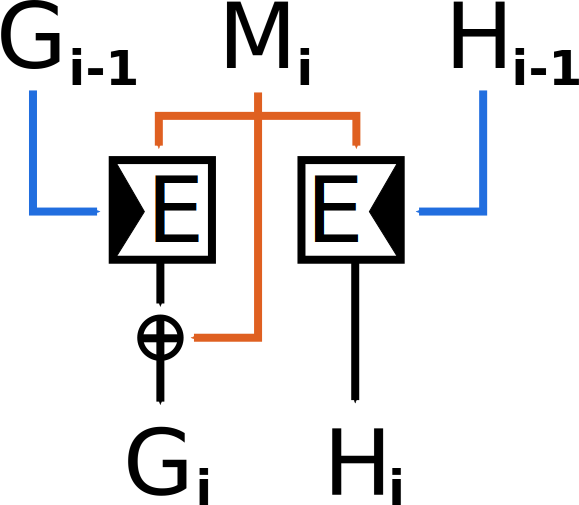
\includegraphics[width=5cm]{drawing.pdf}
\end{figure}

\subsection{The Security of the compression Function}

\begin{description}
    \item \textbf{Collision-security:}
    \item \textbf{Preimage-security:}
    \item \textbf{2nd-Preimage-security:}
\end{description}

\subsection{The Security of the Hash Function}

\begin{description}
    \item \textbf{Collision-security:} Since $H_0$ is fixed and $E$ is invertible it is impossible that different $M_1$ collide.
    \item \textbf{Preimage-security:} As there are no collisions with this structure, no preimages exist at all.
    \item \textbf{2nd-Preimage-security:} Due to the invertibility of $E$, it's easy to calculate $M_1 = E_{H_0}^{-1}(H_1)$
\end{description}

\end{document}
